\documentclass[specialist,
               %substylefile = spbu.rtx,
               subf,href,colorlinks=true, 12pt,a4paper]{article} %href
\usepackage[utf8]{inputenc} 
\usepackage[english,russian]{babel} 
\usepackage{indentfirst}
\usepackage[a4paper,
            mag=1000, includefoot,
            left=3cm, right=1.5cm, top=2cm, bottom=2cm, headsep=1cm, footskip=1cm]{geometry}
\usepackage{amsfonts}
\usepackage{amsmath}
\usepackage{amsthm}
\usepackage{multirow}
\usepackage{rotating} 
\usepackage{longtable}
%\usepackage{slashbox}
\newcommand{\R}{\mathbb{R}}
\newcommand{\N}{\mathbb{N}}
\newcommand{\E}{\mathbb{E}}
\newcommand{\D}{\mathbb{D}}
\newcommand{\T}{\mathrm{T}}
\usepackage[T2A]{fontenc}
\numberwithin{equation}{section}
\pagestyle{plain}
\usepackage{natbib}
\usepackage{caption}
\newcommand{\scal}[2]{\left\langle #1,#2 \right\rangle}
\makeatletter
\long\def\theequation{\ifnum \c@section > 0 \thesection .\else \thechapter .\fi  \@arabic \c@equation}
\makeatother

%\chapterpagestyle{footcenter}

%\usepackage{chngcntr}
%\counterwithout{section}{chapter}
%\setcounter{chapter}{0}
%\counterwithin{section}{section}
\newtheorem{mydef}{Определение}
\newtheorem{mytheor}{Теорема}
%%%%%%%%%%%%%%%%%%%
%\ifx\pdfoutput\undefined
%\usepackage{graphicx}
%\else
%\usepackage[pdftex]{graphicx}
%\fi

%%%%%%%%%%%%%%%%
\usepackage[T2A]{fontenc}
\ifpdf\usepackage{epstopdf}\fi

% Точка с запятой в качестве разделителя между номерами цитирований
%\setcitestyle{semicolon}

% Использовать полужирное начертание для векторов
\let\vec=\mathbf

% Включать подсекции в оглавление
\setcounter{tocdepth}{2}

\usepackage[labelsep=none]{caption}
\DeclareCaptionLabelFormat{figure}{\hspace{15pt}\textbf{\figurename\nobreakspace\thefigure.~}}
\captionsetup[figure]{labelformat=figure}
\DeclareCaptionLabelFormat{tableformat}{\hspace{15pt}\textbf{\tablename\nobreakspace\thetable.~}}
\captionsetup[table]{labelformat=tableformat}


\graphicspath{{fig/}}

%----------------------------------------------------------------
\begin{document}


	\thispagestyle{empty}
%
	\begin{center}
		Санкт-Петербургский государственный университет \\
		\vspace{0.3cm}	
		Прикладная математика и информатика \\
		\vspace{0.3cm}
		Кафедра статистического моделирования \\
		
		\vspace{8cm}		
			Ширинкина Дарья Андреевна \\
		{\large 
		   	
			
			\vspace{0.3cm}	
			%\vspace{2cm}	
			\Large Регуляризация в регрессии \\
			\vspace{12cm}	

		}
		Санкт-Петербург \\
				2017
	\end{center}
	
\newpage


\tableofcontents
\newpage

%\intro
\section{Задача регрессии}
\subsection{Задача регрессии на генеральном языке}

Предполагаем, что существует неизвестная зависимость $f: \R^p \rightarrow \R$ между случайными величинами $\eta \in \R$ и $\xi \in \R^p$:

\begin{equation*}
\eta = f(\xi) + \epsilon,
\end{equation*}

где $\epsilon$ --- случайная величина (ошибка) такая, что $\xi$ и $\epsilon$ независимы. Будем считать также, что $\E\epsilon = 0$ и $\E \epsilon^2 = \sigma^2$.

\textbf{Задача:} хотим оценить функцию $f$.

\subsection{Задача регрессии на выборочном языке}

На практике имеем выборку размера $n$ из случайной величины $\xi$: $X = [X_1, \ldots, X_p]$, где $X_j = (x_{1j}, \ldots, x_{nj})^{\T}$, $j = 1, \ldots, p$. На этой выборке известны результаты функции $f$, то есть имеем выборку $Y = (y_1, \ldots , y_n)^{\T}$ из случайной величины $\eta$ и выборку $\varepsilon = (\varepsilon_1, \ldots , \varepsilon_n)$ из случайной величины $\epsilon$.

Пусть $x_i = (x_{i1}, \ldots, x_{ip})$, тогда запишем зависимость $f$ следующим образом:

\begin{equation*}
y_i = f(x_i) + \varepsilon_i.
\end{equation*}

Хотим по имеющейся выборке $X$ оценить функцию $f$.


\subsection{Линейная регрессия и МНК}

Будем называть выборку $(x_1, \ldots, x_n)^{\T}$, участвующую  в оценке функции $f$, обучающей выборкой и при $i = 1, \ldots, n$

\begin{equation*}
y_i = f(x_i) + \varepsilon_i.
\end{equation*} 

Будем называть выборку  $(x_1', \ldots, x_k')^{\T}$, не участвующую в оценке функции $f$, тестовой выборкой и при $i = 1, \ldots, n$
\begin{equation*}
y_i' = f(x_i') + \varepsilon_i'.
\end{equation*} 



Далее будем предполагать, что рассматриваемая зависимость --- линейная. Считаем, что $Y = (y_1, \ldots, y_n)^{\T}$ и $X = [X_1, \ldots ,X_p]$ --- центрированы. Тогда модель многомерной линейной регрессии можно записать следующим образом:

\begin{equation*}
y_i = f(x_i, \beta) + \varepsilon_i = \sum_{j=1}^p \beta_j x_{ij} + \varepsilon_i,
\end{equation*}

где $\beta = (\beta_1, \ldots, \beta_p)^{\T} \in \R^p$ --- параметры функции $f$.

Процесс подбора оптимального параметра $\beta$ по обучающей выборке $X$ называют обучением. Для оценки параметра $\beta$ будем минимизировать среднюю квадратичную ошибку (МНК)

\begin{equation*}
\mathrm{MSE}_{\mathrm{training}} = \frac{1}{n}\sum_{i=1}^n(y_i - \sum_{j=1}^p \beta_j x_{ij})^2 \rightarrow \min_{\beta}.
\end{equation*}

Решением метода наименьших квадратов (МНК) является вектор

\begin{equation*}
\hat{\beta} = (X^{\T}X)^{-1} X^{T}Y
\end{equation*}

и оценкой функции $f$, когда $f$ --- линейная функция, является  

\begin{equation*}
\hat{f}(x_i) = \sum_{j=1}^p \hat{\beta}_j x_{ij}.
\end{equation*}

\subsection{Проблема МНК}

Метод наименьших квадратов минимизирует среднюю квадратичную ошибку для обучающей выборки, но это не гарантирует, что на тестовой выборке $\hat{f}$ будет также минимизировать среднюю квадратичную ошибку

\begin{equation*}
\mathrm{MSE}_{\mathrm{test}} = \frac{1}{n}\sum_{i=1}^n(y_i' - \sum_{j=1}^p \beta_j x_{ij}')^2.
\end{equation*}

Когда оценка $\hat{f}$ дает ошибку больше на новых объектах, не участвовавших в обучении, чем на обучающей выборке ($\mathrm{MSE}_{\mathrm{test}} \gg \mathrm{MSE}_{\mathrm{training}}  $) говорят, что происходит переобучение. 

По мере увеличения количества параметров модели значение $\mathrm{MSE}_{\mathrm{training}}$ будет уменьшаться, а $\mathrm{MSE}_{\mathrm{test}}$ нет. Это происходит потому что метод обучения будет сильно усложняться и пытаться объяснить то, что вызвано случайностью, а не свойствами функции~$f$.

Рассмотрим от чего зависит $\mathrm{MSE}_{\mathrm{test}}$ на генеральном языке. Пусть
\begin{itemize}
\item $x_i'$ --- реализация случайной величина из тестовой выборки;
\item $y_i' = f(x_i') + \varepsilon_i'$ --- известное значение.
\end{itemize}
Тогда математическое ожидание квадрата ошибки для $x_i'$

\begin{equation*}
\E(y_i' - \hat{f}(x_i'))^2 = Var(\hat{f}(x_i')) + (Bias(\hat{f}(x_i')))^2 + Var(\varepsilon_i').
\end{equation*}

Таким образом, ошибка для объекта, не участвовавшего в обучении, зависит от дисперсии оценки функции $f$ и квадрата смещения. Дисперсия оценки определяет то количество, на которое изменится $\hat{f}$, если бы мы получали эту оценку с использованием другого набора данных. Мы хотим, чтобы оценка $\hat{f}$ не менялась сильно на разных обучающих выборках. Смещение $\hat{f}$ характеризует ошибку, возникающую при аппроксимации реальной сложной функции $f$ более простой моделью.

Как правило, при увеличении сложности метода (увеличение числа параметров) дисперсия будет увеличиваться, а смещение будет уменьшаться. За счет введения в оценку небольшого смещения, можно значительно уменьшить ее дисперсию и тем самым уменьшить $\mathrm{MSE}_{\mathrm{test}}$.

В случае многомерной линейной регрессии оценка $\hat{f}$ не имеет смещения, так как нет смещения у оценки $\hat{\beta}$. Но чем больше дисперсия оценки $\hat{\beta}$ 

\begin{equation*}
\mathrm{Cov}(\hat{\beta}) = \sigma^2(X^{\T}X)^{-1},
\end{equation*}
тем больше дисперсия $\hat{f}$. Когда матрица $X$ близка к вырожденной, дисперсия $\hat{\beta}$ становится большой и $\mathrm{MSE}_{\mathrm{test}}$ увеличивается.


\section{Гребневая регрессия}

\subsection{Задача гребневой регрессии}

Чтобы ввести смещение оценке параметра $\beta$ добавим в $\mathrm{MSE}_{\mathrm{training}}$ множитель, который будет ограничивать параметр $\beta$. Тогда задача минимизации будет выглядеть следующим образом:

\begin{equation*}
\sum_{i=1}^n(y_i - \sum_{j=1}^p \beta_j x_{ij})^2  + \lambda \sum_{j = 1}^p \beta_j^2 \rightarrow \min_{\beta},
\end{equation*}
где $\lambda \geq 0$ --- неотрицательный параметр регуляризации (tuning parameter). Такая модель минимизирует среднюю квадратичную ошибку, но при этом второй множитель $\lambda\sum_{j = 1}^p \beta_j^2$ мал, когда параметры $\beta_1, \ldots, \beta_p$ близки к нулю. 

При $\lambda = 0$, то гребневая регрессия совпадает с обычной регрессией, но при $\lambda \rightarrow \infty$ коэффициенты регрессии стремятся к нулю. Таким образом, для каждого значения $\lambda$ будем получать свой оптимальный набор параметров $\beta_1, \ldots, \beta_p$, поэтому для уменьшения $\mathrm{MSE}_{\mathrm{test}}$ важно подобрать хорошее значение параметра $\lambda$. 

\subsection{Решение задачи минимизации и выбор параметра регуляризации}


Решение гребневой регрессии можно выписать в явном виде:

\begin{equation}\label{greb_regr_min_fun}
\hat{\beta}_{\lambda}^{R} = (X^{\mathrm{T}}X+ \lambda I_p)^{-1} X^{\mathrm{T}}Y.
\end{equation}

Запишем модифицированное МНК решение гребневой регрессии через сингулярное разложение матрицы $X = VDU^{\T}$, где матрицы $V$ размера $n \times p$ и $U$ размера $p \times p$ --- ортогональные, а матрица $D = \mathrm{diag}(\lambda_1, \ldots, \lambda_p)$ --- диагональная, на диагонали которой стоят собственные числа матрицы $X^{\T}X$.

Тогда решение МНК:
\begin{equation*}
\hat{\beta} = \sum_{j=1}^p \frac{1}{\sqrt{\lambda_j}} U_j(V_j^{\T}Y).
\end{equation*}

Решение гребневой регрессии:
\begin{equation}\label{greb_regr_solution}
\hat{\beta}_{\lambda}^{R} = U(D^2 + \lambda I_p)^{-1}DV^{\T}y = \sum_{j=1}^p \frac{\sqrt{\lambda_j}}{\lambda_j + \lambda} U_j(V_j^{\T}Y).
\end{equation}

При этом оценка функции $f$ для выборки $X$ запишется следующим образом:

\begin{equation}\label{grep_regr_f}
X\hat{\beta}_{\lambda}^{R} = VDU^{\T}\hat{\beta}_{\lambda} = V \mathrm{diag}(\frac{\lambda_j}{\lambda_j + \lambda}) V^{\T}Y = \sum_{j=1}^p \frac{\lambda_j}{\lambda_j + \lambda} V_j(V_j^{\T}Y).
\end{equation}

Такой способ записи решения задачи минимизации удобен для выбора параметра $\lambda$.  Выражение \eqref{greb_regr_min_fun} можно переписать, используя  \eqref{greb_regr_solution} и \eqref{grep_regr_f}. Таким образом, необходимо один раз произвести сингулярное разложение матрицы $X$, а затем несложным образом вычислять функционал \eqref{greb_regr_min_fun} для интересующих значений параметра $\lambda$. 

Как выбрать параметр $\lambda$:
\begin{enumerate}
\item выбираем сетку значений $\lambda$;
\item вычисляем ошибку кросс-проверки для каждого значения $\lambda$, используя запись \eqref{greb_regr_min_fun} через сингулярное разложение;
\item выбираем $\lambda$ с наименьшим значением ошибки кросс-проверки;
\item перестраиваем модель со всеми наблюдениями с выбранным значением $\lambda$.
\end{enumerate}


\subsection{Свойства и проблемы}

\textbf{Свойства:}
\begin{enumerate}
\item Рассмотрим вероятностную интерпретацию гребневой регрессии. Предполагая, что

\begin{itemize}
\item $\beta = (\beta_1, \ldots, \beta_p)^{\T}$ имеет априорное распределение $p(\beta)$;
\item $f(Y|X,\beta)$ --- функция правдоподобия исходных данных;
\item линейная модель имеет независимые и нормально распределенные ошибки; 
\item $p(\beta) = \prod_{j = 1}^p g(\beta_j)$ для некоторой плотности $g$.
\end{itemize}

По теореме Байеса при фиксированном $X$ апостериорное распределение $p(\beta|X,Y)$ пропорционально $f(Y|X,\beta)p(\beta|X) = f(Y|X,\beta)p(\beta)$ и если $g$ --- плотность $N(0,\lambda)$, то  оценка апостериорного максимума $\beta$ совпадает с решением гребневой регрессии.

\item Так как решение гребневой регрессии можно выписать в явном виде \eqref{greb_regr_solution}, то покажем, что оценка $\beta$ имеет смещение. Пусть $X^{\T}X = \Sigma$ и $Y = (y_1, \ldots, y_n)^{\T}$, тогда

\begin{align*}
\hat{\beta}_{\lambda}^R &= (X^{\T}X + \lambda I_p)^{-1}X^{\T}Y = \\
 &= (\Sigma + \lambda I_p)^{-1} \Sigma(\Sigma^{-1}X^{\T}Y) = \\
 &= [\Sigma(I_p + \lambda\Sigma^{-1})]^{-1} \Sigma[(X^{\T}X)^{-1}X^{\T}Y] = \\
 &= (I_p + \lambda \Sigma^{-1})^{-1} \Sigma^{-1} \Sigma \hat{\beta} = \\
 &= (I_p + \lambda \Sigma^{-1})\hat{\beta}.  
\end{align*}

Посчитаем математическое ожидание

\begin{align*}
\E\hat{\beta}_{\lambda}^{R} &= \E[(I_p + \lambda \Sigma^{-1})\hat{\beta}] = \\
	&= (I_p + \lambda \Sigma^{-1})\beta.
\end{align*} 

При $\lambda = 0$ оценка совпадает с МНК оценкой и не имеет смещения.
\end{enumerate}

\textbf{Проблемы:}
\begin{enumerate}
\item Оценки МНК инварианты относительно умножения признака на константу, то есть значение $f(x_j)\hat{\beta_j}$ не зависит от масштаба $j$-го признака. В случае гребневой регрессии инвариант относительно масштаба теряется, оценки МНК гребневой регрессии могут сильно измениться при умножении заданного признака на константу. Поэтому гребневую регрессию нужно использовать после стандартизации признаков.
\item В конечную модель входят все начальные признаки, если признаков много, то усложняется интерпретация. 
\end{enumerate}

\section{Лассо}

\subsection{Задача минимизации Лассо}

Метод Лассо, как и гребневая регрессия, вводит смещение у оценки $\beta$, при этом в конечную модель Лассо могут входить не все начальные признаки, что решает проблему гребневой регрессии. Это происходит за счет другого множителя в задачи минимизации, который регулирует коэффициенты $\beta_1, \ldots, \beta_p$, однако из-за этого усложняется решение задачи. Задача минимизации Лассо:

\begin{equation}\label{lasso_min_fun}
\sum_{i=1}^n(y_i - \sum_{j=1}^p \beta_j x_{ij})^2 + \lambda \sum_{j = 1}^p |\beta_j| \rightarrow \min_{\beta},
\end{equation}
где $\lambda \geq 0$ --- неотрицательный параметр регуляризации (tuning parameter). Как и в гребневой регрессии $\lambda \sum_{j = 1}^p |\beta_j|$ мало, когда $\beta_1, \ldots, \beta_p$ близки к нулю. При увеличении параметра $\lambda$ некоторые коэффициенты регрессии становятся равными нулю. Как и в гребневой регрессии необходимо выбрать хорошее значение $\lambda$.


\subsection{Решение задачи минимизации и выбор параметра регуляризации}

Задача минимизации \eqref{lasso_min_fun} эквивалента задаче минимизации с ограничением:

\begin{align*}
\sum_{i=1}^n(y_i - \sum_{j=1}^p \beta_j x_{ij})^2 \rightarrow \min_{\beta}, \qquad  \sum_{j = 1}^p |\beta_j| \leq s,
\end{align*}
где параметру $\lambda$ соответствует параметр $s$. Чем меньше $s$, тем больше нулевых значений коэффициентов $\beta$. Такую задачу можно решить, так как это задача квадратичного программирования. 

Значение параметра $\lambda$ выбирается как в гребневой регрессии с помощью кросс-проверки.


\subsection{Свойства}


\textbf{Свойства:}
\begin{enumerate}
\item Рассмотрим вероятностную интерпретацию Лассо. Предполагая, что

\begin{itemize}
\item $\beta = (\beta_1, \ldots, \beta_p)^{\T}$ имеет априорное распределение $p(\beta)$;
\item $f(Y|X,\beta)$ --- функция правдоподобия исходных данных;
\item линейная модель имеет независимые и нормально распределенные ошибки; 
\item $p(\beta) = \prod_{j = 1}^p g(\beta_j)$ для некоторой плотности $g$.
\end{itemize}

По теореме Байеса при фиксированном $X$ апостериорное распределение $p(\beta|X,Y)$ пропорционально $f(Y|X,\beta)p(\beta|X) = f(Y|X,\beta)p(\beta)$ и если $g$ --- плотность распределения Лапласса с нулевым средним и параметром масштаба $\lambda$, то оценка апостериорного максимума $\beta$ является решением Лассо. 

\item Лассо обнуляет некоторые коэффициенты $\beta_1, \ldots, \beta_p$. Задачу минимизации гребневой регрессии можно также рассмотреть в виде 

\begin{align*}
\sum_{i=1}^n(y_i - \sum_{j=1}^p \beta_j x_{ij})^2 \rightarrow \min_{\beta}, \qquad  \sum_{j = 1}^p \beta_j^2 \leq s.
\end{align*}

Рассмотрим простой случай, когда $p = 2$. Тогда выражение $\sum_{i=1}^n(y_i - \sum_{j=1}^p \beta_j x_{ij})^2$ будет представлять собой эллипс, центр которого находится в точке $\hat{\beta}$ (см. рис.~\ref{lasso_pic}). Предположим, что центр эллипса не удовлетворяет ограничениям $\sum_{j = 1}^p \beta_j^2 \leq s$ и $\sum_{j = 1}^p |\beta_j| \leq s$, то есть лежит вне круга в случае гребневой регрессии и вне ромба в случае Лассо. Тогда решения задач минимизации будет лежать на границе возможных значений. Данная ситуация изображена на рис.~\ref{lasso_pic}, можно заметить, что для Лассо существует гораздо больше различных эллипсов, которые пересекались бы с ромбом (ограничениями) таким образом, чтобы один из коэффициентов был равен нулю.

\begin{figure}[h]\label{lasso_pic}
\center{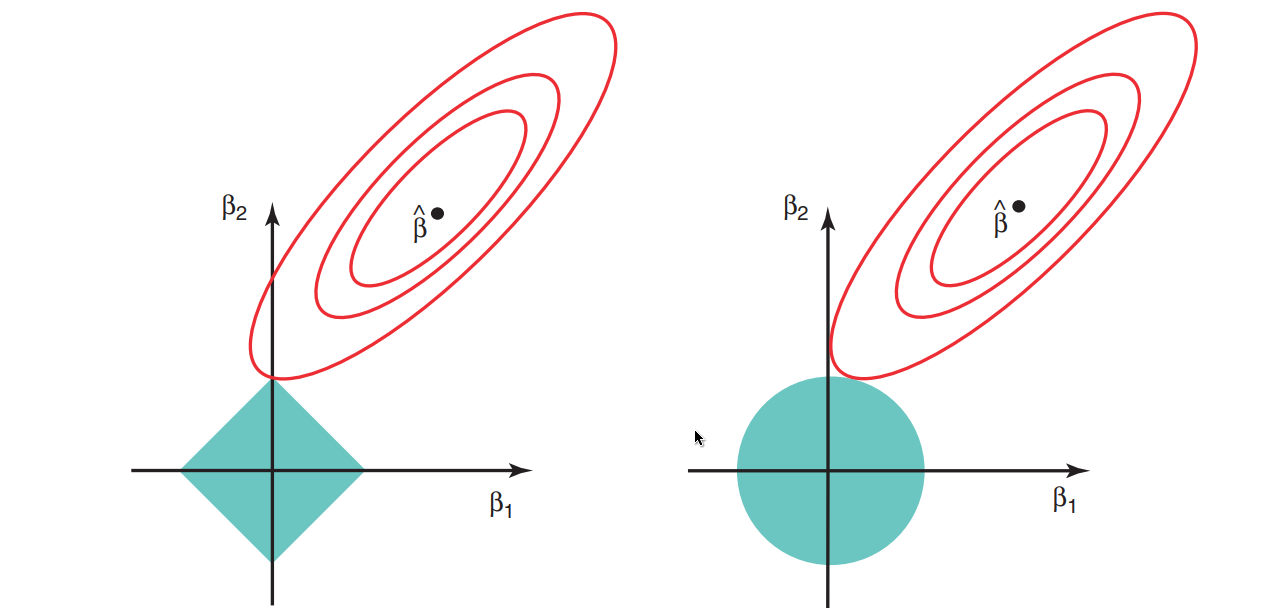
\includegraphics[width=1\linewidth]{Lasso_and_ridge.png}}
\caption{Границы ошибки $\sum_{i=1}^n(y_i - \sum_{j=1}^p \beta_j x_{ij})^2$ и ограничений  $\sum_{j = 1}^p |\beta_j| \leq s$ для Лассо (слева) и $\sum_{j = 1}^p \beta_j^2 \leq s$ для гребневой регрессии (справа).}
\label{lasso_pic}
\end{figure}
\end{enumerate}

\newpage

\section{Сравнение гребневой регрессии и Лассо}

Рассмотрим простой случай, когда $n = p$ и $X$ --- диагональная матрица с $1$ на диагонали. Тогда задача минимизации для обычной регрессии принимает вид

\begin{equation*}
\sum_{j =1}^p (y_j - \beta_j)^2.
\end{equation*}

Решение МНК:

\begin{equation*}
\hat{\beta}_j = y_j.
\end{equation*}


Решение гребневой регрессии будет принимать вид:
\[\hat{\beta}_{\lambda}^R = \frac{y_j}{1 + \lambda}.\]

Решение Лассо:
\begin{equation*}
\hat{\beta}_{\lambda}^L = 
 \begin{cases}
   y_j - \lambda/2, & \qquad y_j > \lambda/2\\
   y_j + \lambda/2, & \qquad y_j < -\lambda/2 \\
   0, & \qquad |y_j| \leq \lambda/2.
 \end{cases}
\end{equation*}


Рисунок~\ref{comparing} иллюстрирует разный подход к регулированию коэффициентов $\beta_1, \ldots, \beta_p$. Гребневая регрессия уменьшает каждый коэффициент с равной пропорцией. Лассо уменьшает значения коэффициентов на одинаковое значение, при этом если коэффициент по модулю меньше $\lambda/2$, то его значение становится равным нулю. В случае более общей матрицы $X$ ситуация немного сложнее, но принцип регуляризации сохраняется. 

В целом нельзя выделить ни одну из моделей (Лассо или гребневая регрессия) как лучшую. С помощью кросс-проверки можно определить какой подход лучше.

\begin{figure}[h]
\center{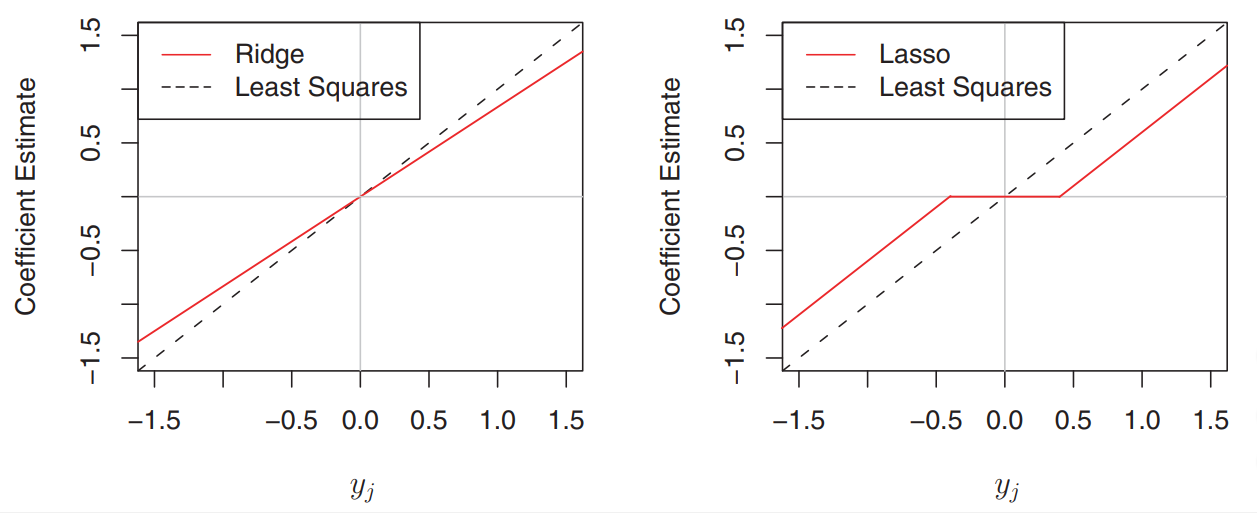
\includegraphics[width=1\linewidth]{compare.png}}
\caption{Случай $n = p$. Слева сравнение МНК и гребневой регрессии. Справа сравнение МНК и Лассо.}
\end{figure}
\label{comparing}
\vspace{-0.3cm}

%\bibliographystyle{gost2008}
%\bibliography{bibl}

\end{document}
